\documentclass[handout]{beamer}

%\usepackage{pgfpages}
%%\setbeameroption{show notes}
%\setbeameroption{show notes on second screen=right}

\setbeamertemplate{caption}[numbered]

\usepackage{tikz}
\usetikzlibrary{calc, matrix, arrows, automata, shapes, positioning, shadows, trees}
\usepackage{graphicx}
\usepackage{multimedia}
\usepackage[latin1]{inputenc}
\usecolortheme{lily}
\setbeamercovered{transparent}
\usepackage{pgfplots}
\usepackage{pgfplotstable}
\usepackage{color}
\usepackage{subfigure}

\tikzset{basic/.style={draw}}
\tikzset{input/.style={basic, circle}}
\tikzset{bias/.style={basic, rectangle}}
\tikzset{neuron/.style={basic, circle}}
\tikzset{>=stealth, font=\scriptsize}
\tikzset{sectors/.style n args={2}{%
     circle, draw, minimum width=3.444em,
     append after command={%
         \pgfextra{ %
            \draw (\tikzlastnode.north) -- (\tikzlastnode.south);
            \path (\tikzlastnode.center) -- node[] {#1} (\tikzlastnode.west);
            \path (\tikzlastnode.center) -- node[] {#2} (\tikzlastnode.east);
         }
      }
   }
}

% argmax
\newcommand{\argmax}[1]{\underset{#1}{\operatorname{arg}\,\operatorname{max}}\;}

\title[\insertdate]{Binary Classification Using (tensor) LDA}

\author{Awais Bajwa,\\ Shinho Kang,\\ Omar Guti\'errez}
%\institute{@trinogz}
\date{\today}

\begin{document}

\begin{frame}
\titlepage
%Mostly based on \textbf{A Tutorial on Bayesian Nonparametric Models} by Samuel J. Gershman.
\end{frame}
\note{}

\begin{frame}
    \frametitle{Outline} 
    \tableofcontents
\end{frame}
\note{}

\section{Linear Discriminant Analysis}
\begin{frame}{Linear Discriminant Analysis}
    \begin{itemize}
        \item \textbf{Task}: Implement a binary classifier for car detection.
        \item Using (conventional) Linear Discriminant Analysis.
    \end{itemize}
\end{frame}
\note{}

\begin{frame}{Steps}
    \begin{itemize}
        \item Calculate mean $\mu$
            \begin{itemize}
                \item For class 0, class 1, and for the overall dataset
            \end{itemize}
        \item Calculate covariance matrix
            \begin{itemize}
                \item $S_B$ and $S_W$
            \end{itemize}
        \item Calculate projector matrix $w$
    \end{itemize}
\end{frame}
\note{}

\begin{frame}{Determine $w$}
    \begin{itemize}
        \item $w$ is a projection vector that maximally separates the data
    \end{itemize}
\Huge{
\begin{equation}
    \textcolor{red}{w} = 
    \textcolor{gray}{\argmax{w}}
    \frac{\textcolor{brown}{w^TS_Bw}}
    {\textcolor{blue}{w^TS_ww}}
\end{equation}
}
\end{frame}

\begin{frame}{Plot from $S_B$}
    {\centering
    \begin{figure}[H]
        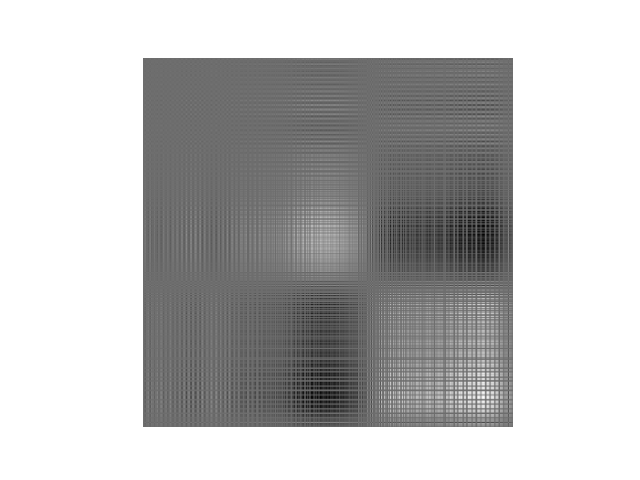
\includegraphics[width=0.75\textwidth]{project_03/s_b.png}
        \caption{Plot from $S_B$}
    \end{figure}
    }
\end{frame}

\begin{frame}{Plot from $S_W$}
    {\centering
    \begin{figure}[H]
        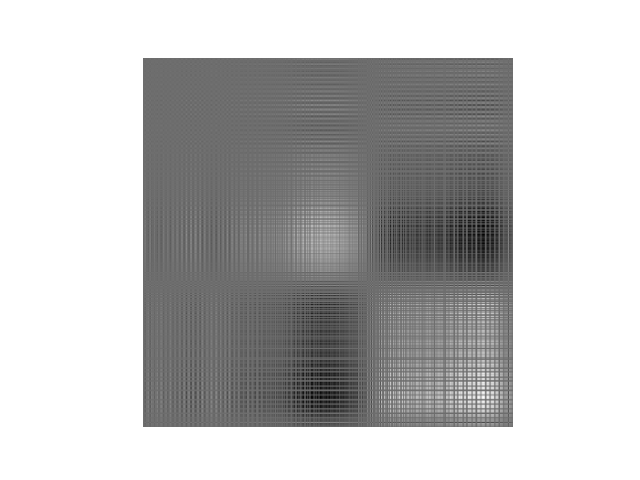
\includegraphics[width=0.75\textwidth]{project_03/s_b.png}
        \caption{Plot from $S_W$}
    \end{figure}
    }
\end{frame}

\begin{frame}{Plot from $w$}
    {\centering
    \begin{figure}[H]
        
\includegraphics[width=0.75\textwidth]{project_03/ww.png}
        \caption{Plot from $w$}
    \end{figure}
    }
\end{frame}

\begin{frame}{Result}
    {\centering
    \begin{figure}[H]
        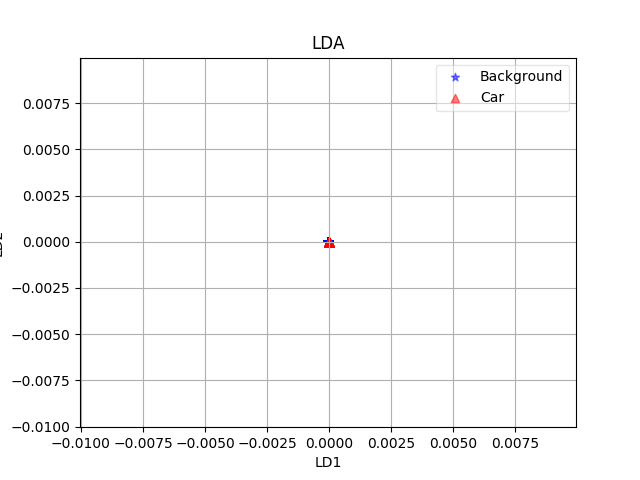
\includegraphics[width=0.75\textwidth]{project_03/lda.png}
        \caption{Result from LDA}
    \end{figure}
    }
\end{frame}

\begin{frame}{Precision and recall}
\Huge
\begin{equation}
    Precision = \frac{tp}{tp + fp}
\end{equation}
\begin{equation}
    Recall = \frac{tp}{tp + fn}
\end{equation}
\end{frame}

\begin{frame}{Precision and recall}
    {\centering
    \begin{figure}[H]
        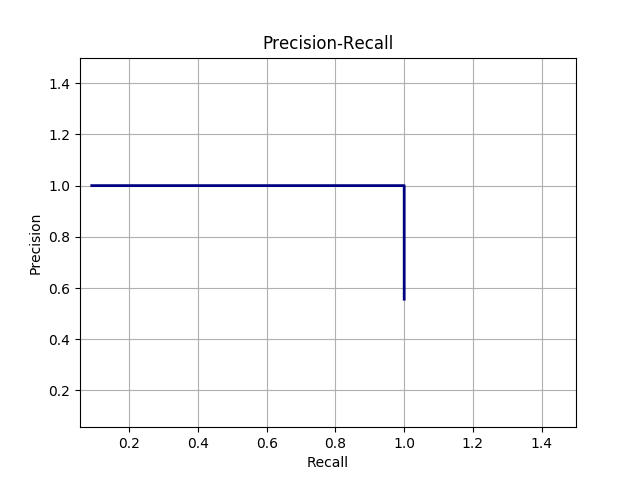
\includegraphics[width=0.75\textwidth]{project_03/precision_recall.png}
        \caption{Precision and recall}
    \end{figure}
    }
\end{frame}

\section{Tensor Linear Discriminant Analysis}
\begin{frame}{Tensor Linear Discriminant Analysis}
    \begin{itemize}
        \item \textbf{Task}: Implement a binary classifier for car detection.
        \item Using Tensor Linear Discriminant Analysis.
    \end{itemize}
\end{frame}
\note{}

\begin{frame}{Tensor W output}
    {\centering
    \begin{figure}[H]
        
\includegraphics[width=0.75\textwidth]{project_03/tensorWOut.jpg}
        \caption{}
    \end{figure}
    }
\end{frame}

\begin{frame}{Determine a projector $w$}
    \Huge
    \begin{equation}
        y(X) = \left\{
                    \begin{tabular}{cc}
                        $+1$, & if $w^{T}x \geq \theta$ \\
                        $-1$, & otherwise
                    \end{tabular}
                \right.
    \end{equation}
\end{frame}

%\begin{frame}
%\huge{Thank you}\\
%\huge{Questions?}\\
%\end{frame}

\end{document}
